%%% -*-LaTeX-*-

\chapter{Results}

In this chapter we evaluate our system using an implementation of the NetFlow host behavior extractor written in python. Our experiments in this section are conducted on a ubuntu16 virtual machine with 80 GB memory and 20 cpus of computing power. 

\section{Dataset: description and clustering}
The traffic analyzed here is collected at the University of Utah's emulab routers \cite{White+:osdi02}, This is a private repository that contains traces of bidirectional traffic into the emulab network and no payload. Traffic is collected on Full Duplex links at a speed of 1Gbps.

We passed the NetFlow records collected over the last 6 months of 2017 through our system to determine the set of behaviors(clusters) hosts exhibited over this time. We have hand picked 7 days of this data for analysis. The chosen days are October 15, October 16, November 14, November 23, December 5, December 12, December 16\footnote{Days are picked without any prior knowledge of any metadata related to NetFlow records}. We made sure that there is a mix of both week days , weekends, normal and heavy traffic days. Each days traffic is treated independently as the same host that appeared on two different days could exhibit different behaviors. For different evaluations in this section we used the data corresponding to the these days.

As mentioned earlier in the section \ref{cluster_labeling} we have choosen a reference day for labeling the clusters. We applied following techniques to label the clusters on the reference day. The first one is port-based analysis to identify applications such as web, mail, and DNS. second one is the anomaly detection methods. Finally, a set of heuristic rules to label manually the behavior of the hosts. After the above steps we found the following clusters. Clusters labeled as T consists of hosts which use few ports on both sides to exchange interactive traffic. Clusters labeled as S consists of hosts which serve clients requests and conversely clusters labeled C consists of hosts which request servers for information. Let us list the differences in these behaviors in detail.

\textbf{Clusters T1-T2} are mostly one-to-one connections, the dominant traffic in these clusters is http/https, ssh and peer to peer traffic. P2P traffic is defined as traffic where hosts uses both TCP and UDP ports concurrently for communication, They also choose arbitary ports for communication. Further analysis, reveals that clusters are split based on packet size and flow size.
While T1 has long living flows with large average packet sizes. T2 has large number of flows which are short lived and an average packet size less than T1.

\textbf{Clusters C1-C2} contains hosts which behave as clients  making connections with different servers, The cluster C2 is dominated by DNS traffic which is in accordance with the heavy DNS requests that the hosts residing in the emulab network make with the external servers (machines outside the Emulab Firewall). Cluster C1 on the other hand comprises of hosts that request for web pages and that have outbound mail traffic.

\textbf{Clusters S1-S2} as mentioned above comprises of hosts that behave as servers which respond to client requests. These hosts generally communicate with different ports of destination machines from a fixed port. S1 cluster contains of majority of hosts which are within emulab network and are acting as servers accepting SSH requests. S2 cluster contains hosts that are both within and outside emulab network which are acting as servers for different sets of traffic such as SSH, Web and DNS which is further explained in the section \ref{cross_validation}. 

\textbf{Cluster A1} is the cluster that is of interest for network security as it contains of hosts that exhibit anamolous behavior trying to scan different access points to enter into the system.

The above description clearly points out that host based behavior extraction produces a richer and finer classification of host behaviors than a port based classifier. For example, Http traffic is split across different clusters T or S which represents how the same protocol can be used differently in real time scenarios. Same is the case with SSH traffic also. While most of these clusters contain hosts using different protocols. They are similar in the sense that each cluster exhibits different functional behavior such as Server, Client or One-to-One traffic.

The \figref{behaviorsdec12} is a comparison between the classification made by a traditional port based classifer(left) and our host based classifier(right). The traditional port based classifier identified the top 8 applications used by the hosts in the system. DNS(53) is the most used application with 11.95\% of the whole traffic trying to query DNS servers. It is followed by Telnet(23), SSH(22) with a share of 9.83\% and 5.08\% traffic respectively. We can also see web traffic both secured and unsecured in the top 8 accounting to 3.84\%, 0.66\% traffic. While, we can see the applications that accounted to majority of traffic by traditional classifier, Our system on the other hand provided an alternate view for the same NetFlow data by extracting the behaviors these hosts are exhibting. From the \figref{behaviorsdec12} we can see that, hosts that are behaving as clients account to 11.41\% (both C1 and C2 combined) of traffic and hosts that are behaving as servers account to 33.61\% (both S1 and S2 combined). The majority of the traffic(50.23\%) comprises of interactive communication between hosts while the anomalous hosts trying to invade into the network form the minority(4.75\%). 

\begin{figure}[t]
	\centerline{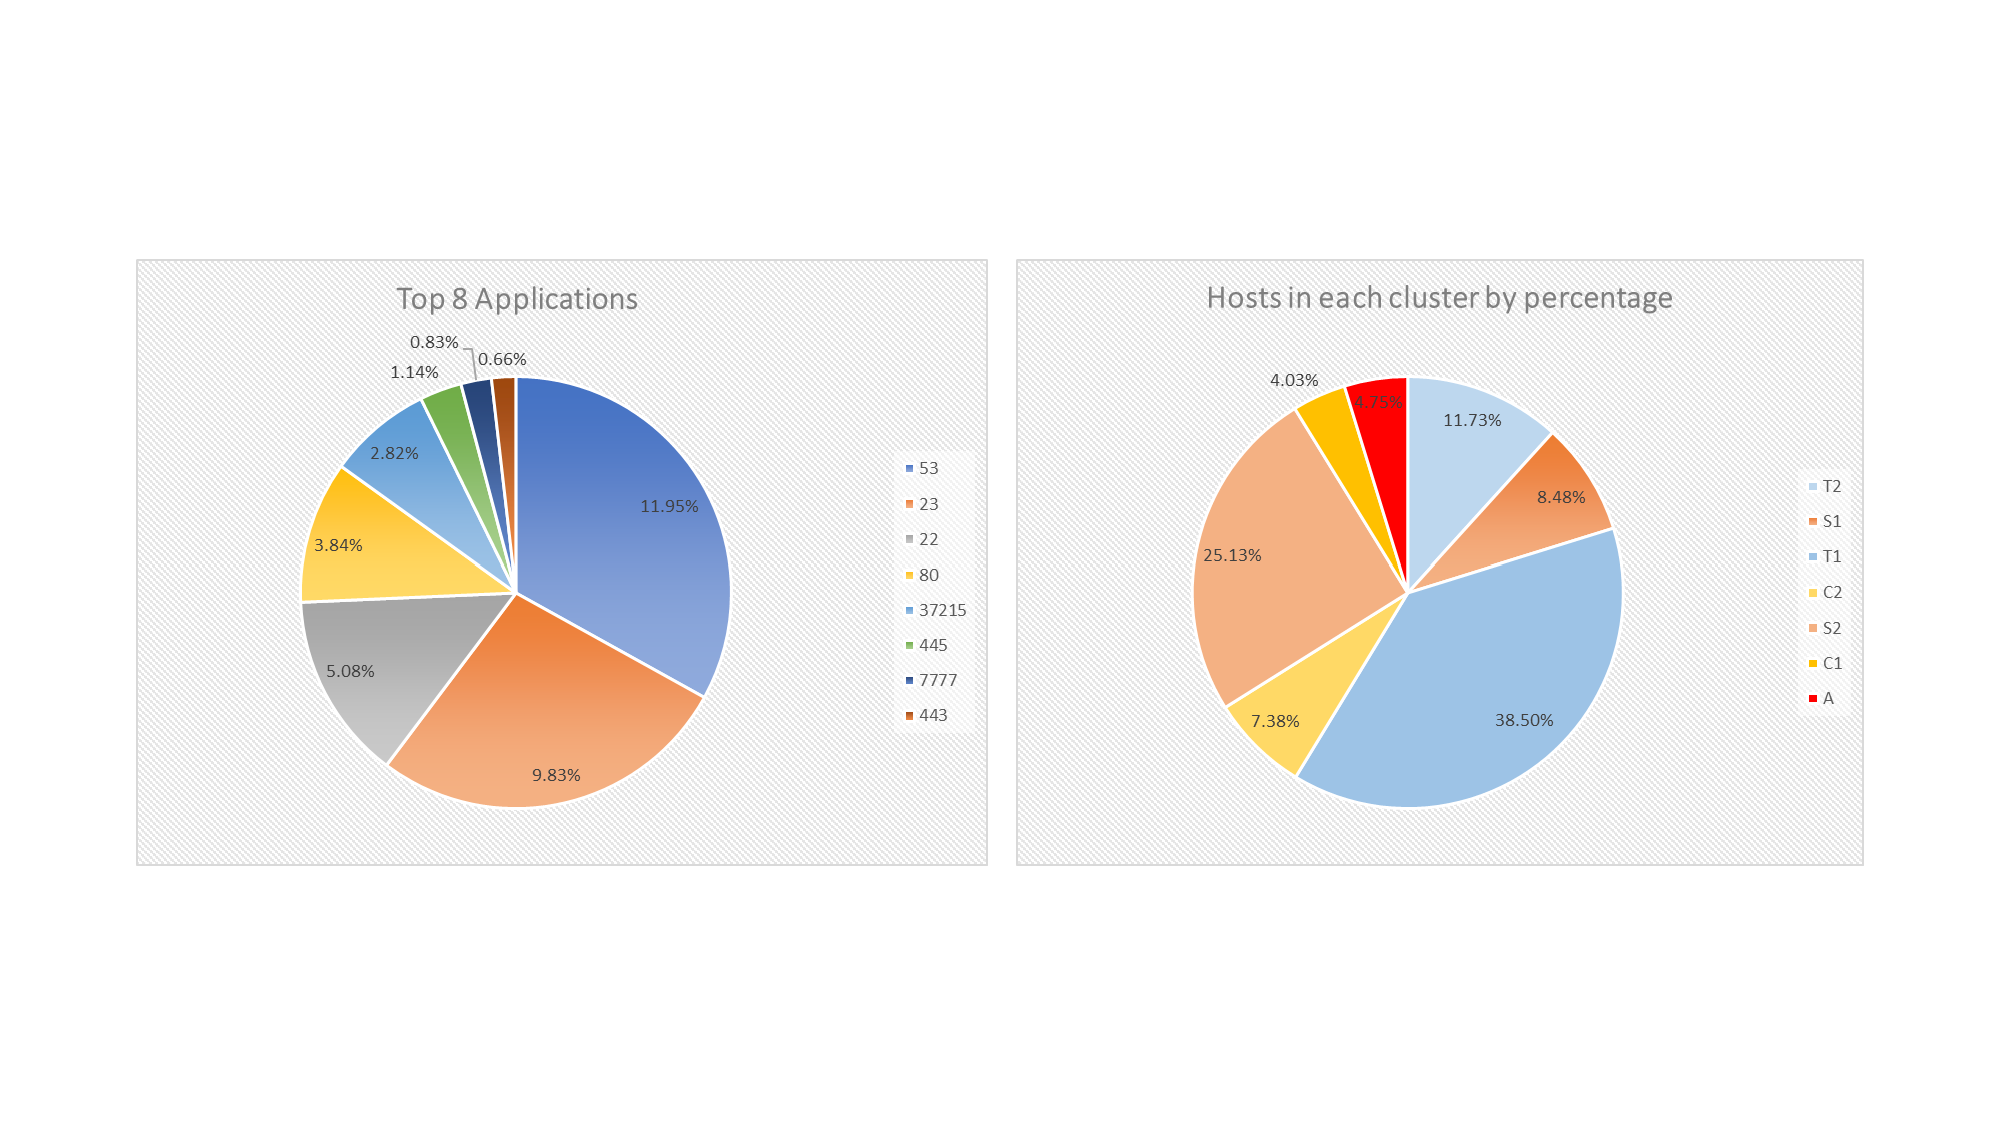
\includegraphics[trim=2cm 2cm 2cm 2cm, scale = 0.5]{dec12-port-behaviors.pdf}}
	\caption{Comparison of hosts using port based classifier (left) and host behavior extractor (right) on December 12, 2017.}%
	\figlabel{behaviorsdec12}
\end{figure}


\section{Cross Validation} \label{cross_validation}
We compared the results obtained from our system with other classification techniques to better understand the significance of our approach.

\textbf{\textit{Cross Validation with a port based classifier}}, We used a classic port based classifying technique to cross validate our results. Though, it isn't a perfect measure and fails in many cases it is good enough to classify a host to a particular class in most of the cases.
In the scenarios when this technique cannot classify a host to particular class we label it as a 'Mix' traffic. The heuristic that we used for labeling as 'Mix' traffic is when the dominant class accounts for less than 50 percent of the traffic by that host. Applying this procedure we observed 20 different classes of traffic, out of which the most frequently observed are discussed here: HTTP, DNS, SSH, MAIL, TELNET, FTP, CHAT, P2P, SMTP, MIX. The cross-validation between the port based approach and  our procedure on one of the choosen day December 12th is reported in \tabref{validation}.

\begin{table}[t]
	\caption{Cross-valdation of the host behavior extraction with port based analysis.}%
	\centerline{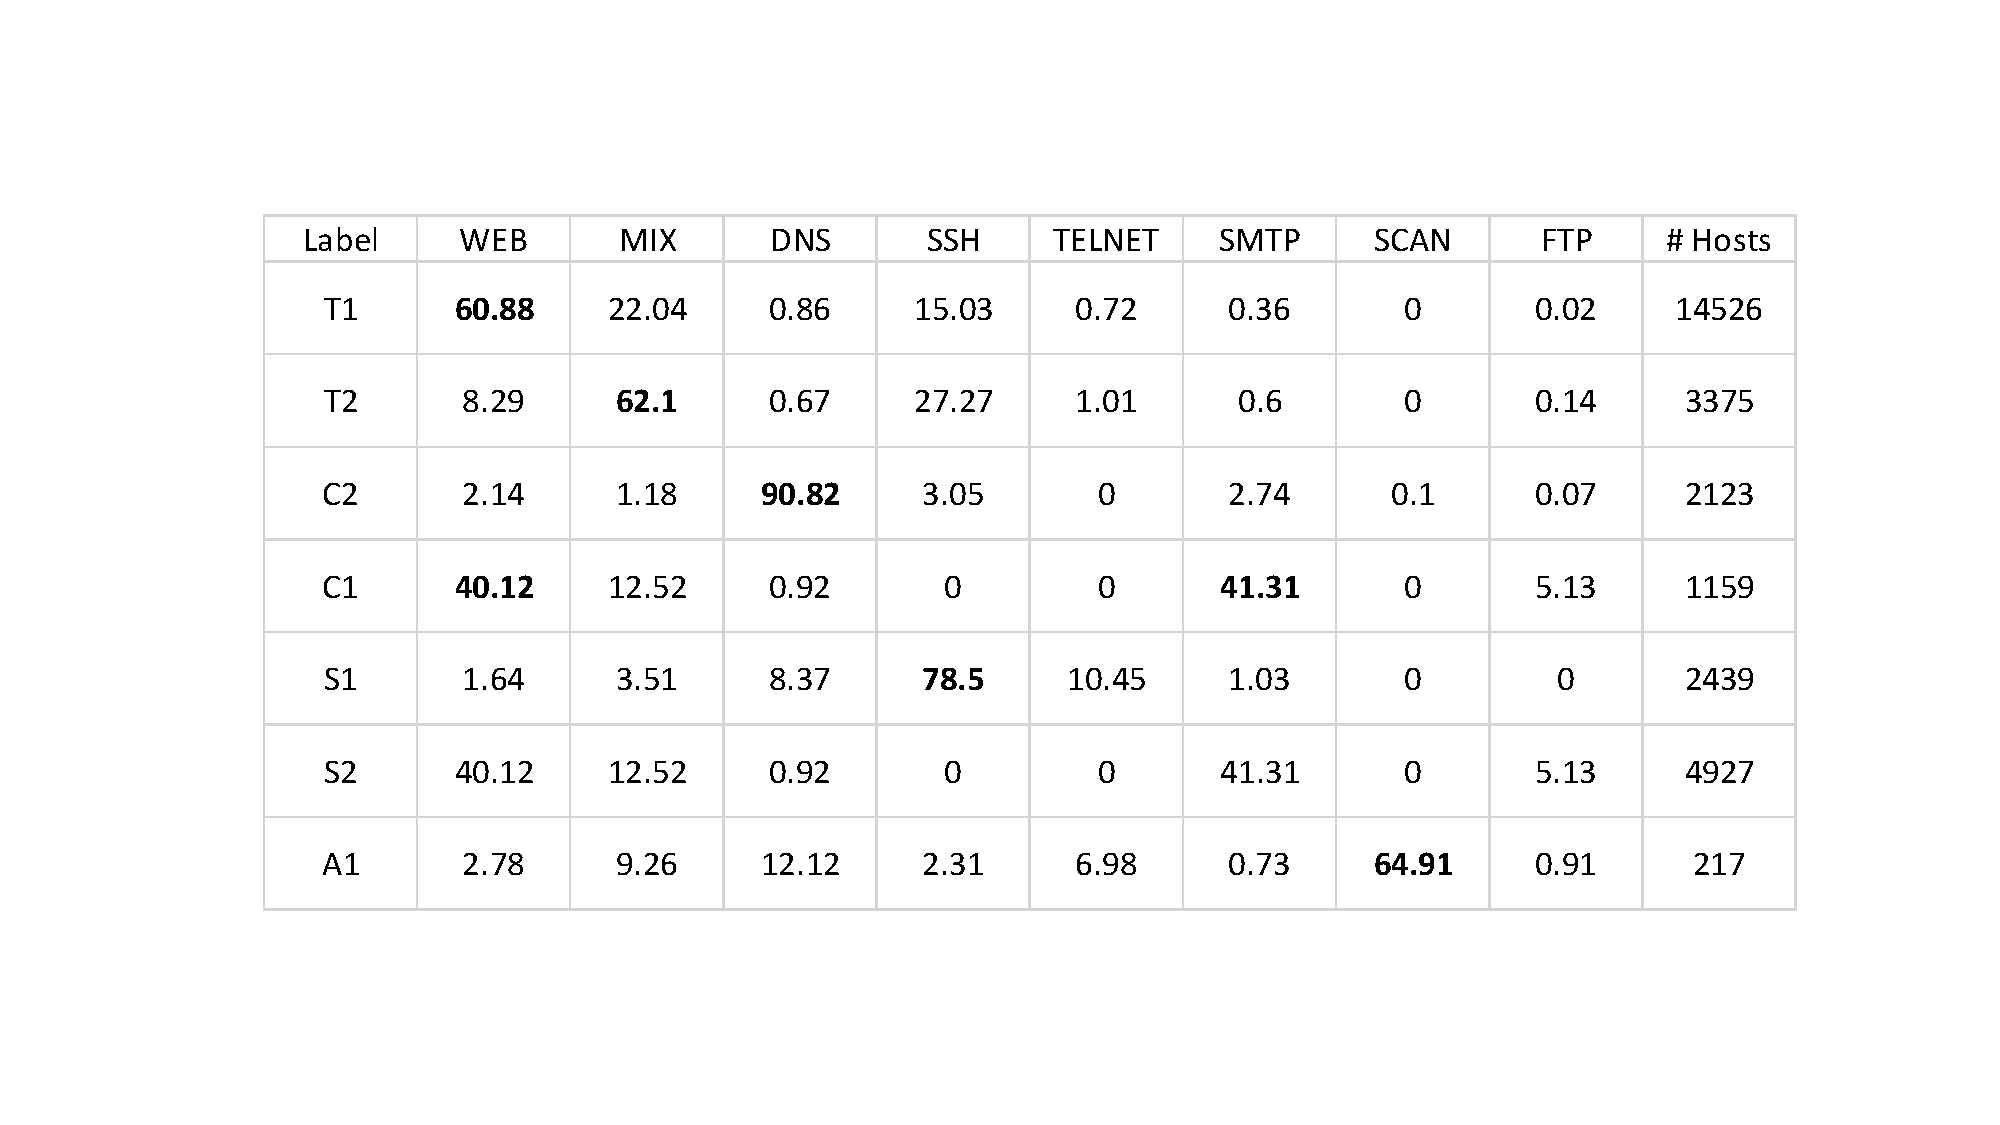
\includegraphics[scale = 0.5]{validation.pdf}}	
	\tablabel{validation}
\end{table}

The row headers in the table correspond to the lables of the clusters generated by our system while the column headers correspond to the different classes of traffic derived by a port based classifier as mentioned above. Each row in the table describes the percentage of hosts within each cluster that fall under different classes of traffic as classified by a port based classifier. For example, in the cluster T1 we have 60.88\% of hosts that are using web applications, 0.86\% of hosts are involved in DNS traffic, 15.03\% of hosts exchange SSH, 0.72\% exchange TELNET traffic and 22.04\% the hosts in this cluster are classified as MIX traffic.
From the highlited parts in the table we can safely conclude that 
we have an high match of host classification which reflects the competence of the proposed procedure. It is also clearly evident from here that the nature of clusters described earlier confirm with the results obtained with cross-validation.This also suggests that all the hosts that fall into a particular class based on port based analysis are not necessarily in the same cluster. They are dispersed across the clusters which shows the necessity of a host based behavior extraction. For example, cluster S1 clearly confirms the fact that the hosts in this cluster are dealing with SSH traffic and the same traffic is also present in T1 and T2 clusters. Similary, hosts in the cluster S2 contains of servers that provide responses for web, ssh and other requests. This cluster has similar distribution as cluster C1 but they act exactly opposite like servers and clients respectively. Also, few points of observation from the table are, T1 has mostly requests and responses between hosts spread across different applications. hosts which are grouped as T2 have most of it's hosts labeled as Mix, which on further investigation revealed that many of the hosts in this class don't pass the majority test to be distinguished into any particular class. Finally, Scanners distribution was minimal across all the clusters. The sparsity of this table also serves as a confident measure for our proposed approach.

The following evaluations also validate our systems results.
Our observation is that the behaviors exhibited by the hosts are quite stable over several months which can be seen in the  \figref{constant}. The graph is a representation of the behaviors exhibited by hosts over a six months of time period. Since we map each cluster to a behavior this is equals to the number of clusters that are formed over a time period. As, we are using K-means clustering, in our case this is a graph drawn between the  value of K on X-axis and the day on which we found this value on Y-axis. Except for few points it is a straight line indicating the constants behaviors that hosts exhibited in our system. Our recommendation is to update the host behaviors every couple of months or as per the change in usage of applications.

\begin{figure}[t]
	\centerline{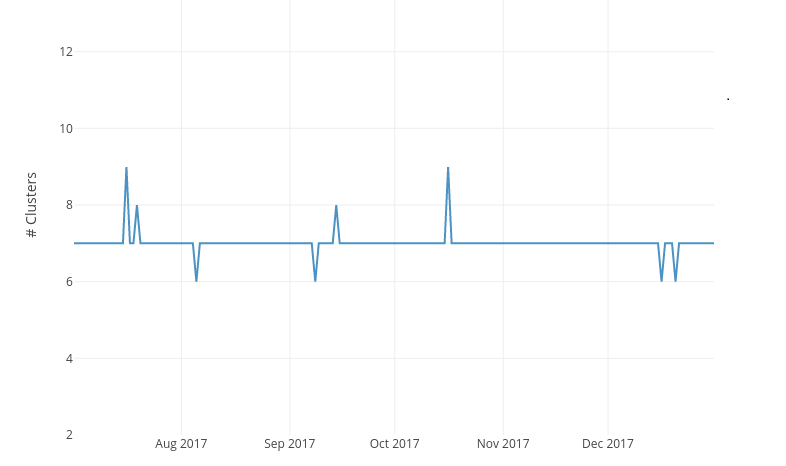
\includegraphics{constant.png}}
	\caption{ Plot of number of clusters formed over a time period.}%
	\figlabel{constant}
\end{figure}


\begin{figure}[t]
	\centerline{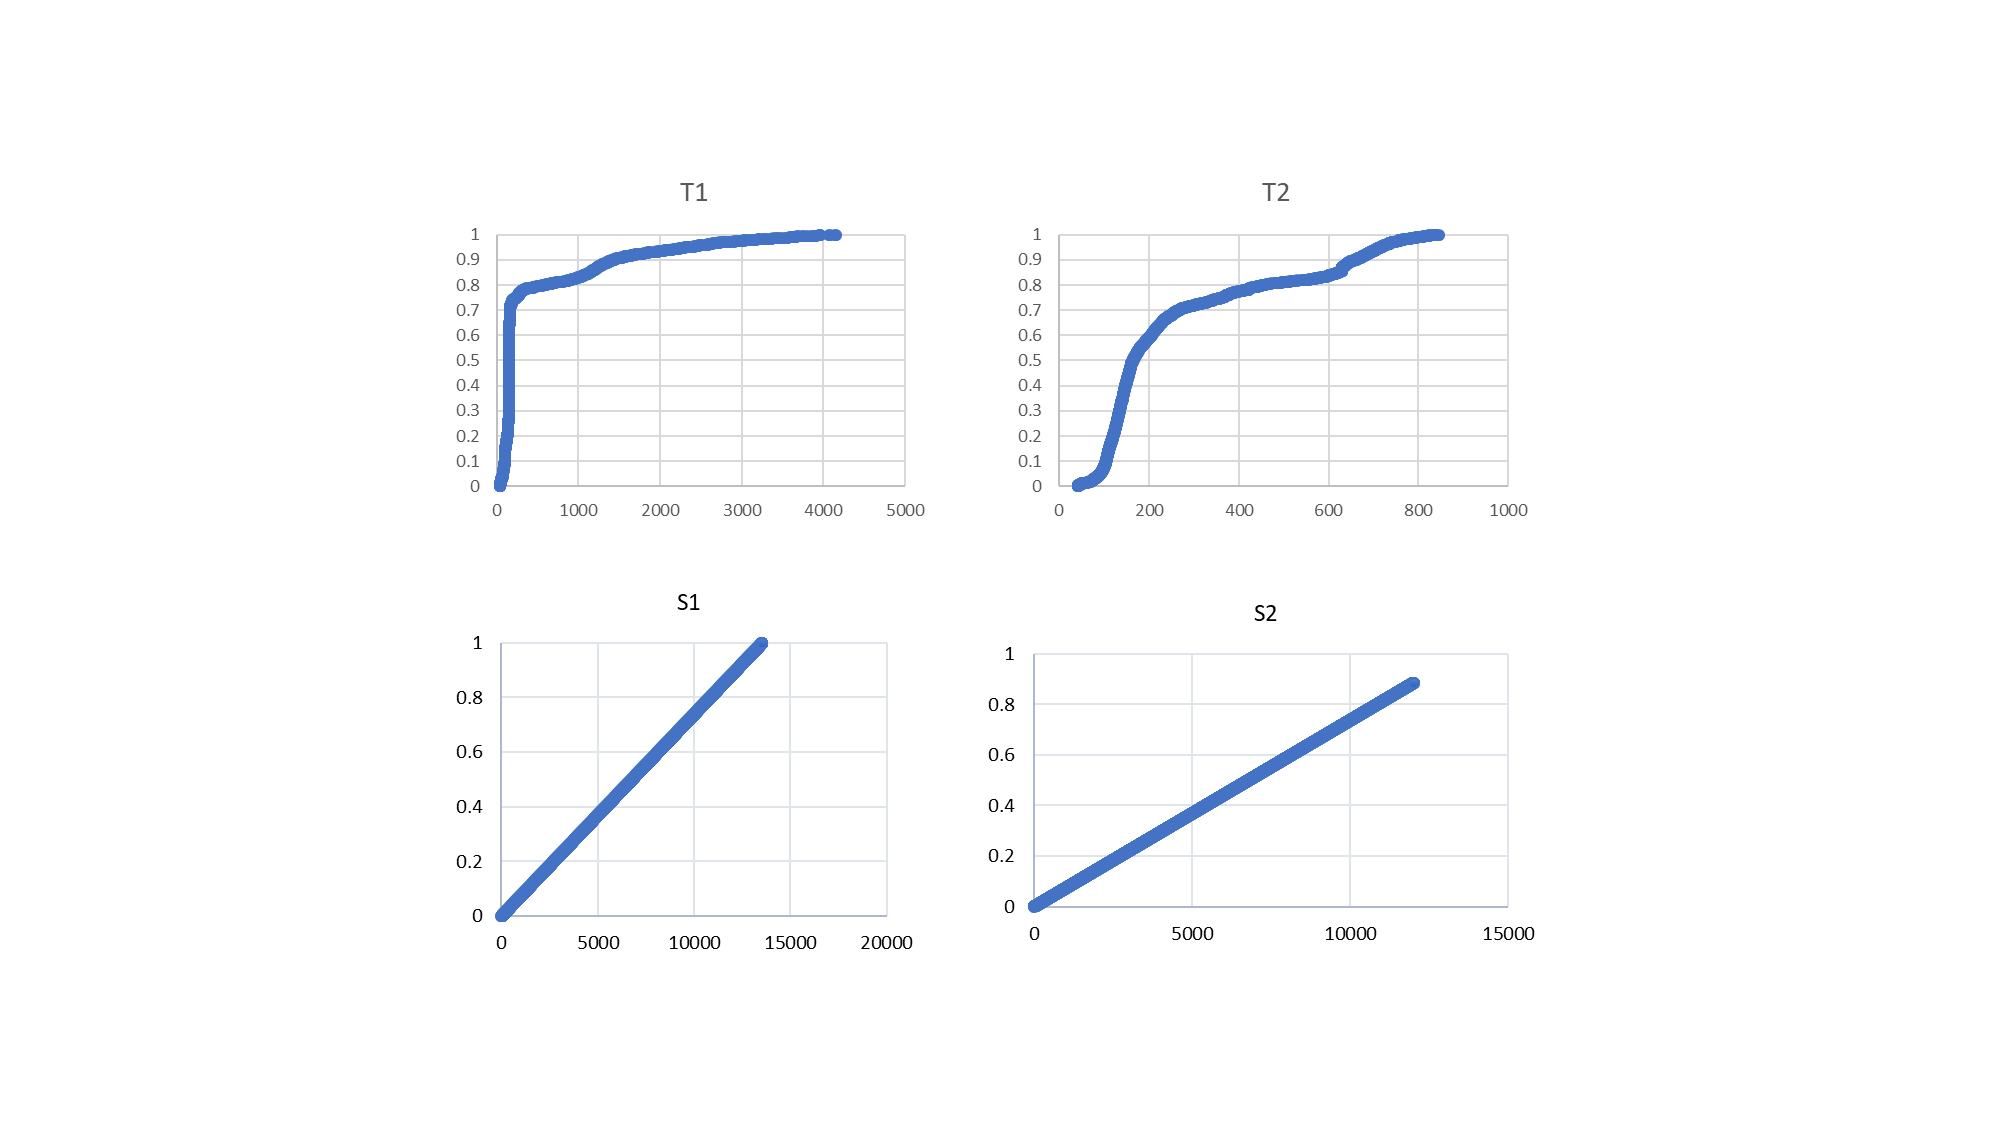
\includegraphics[trim=2cm 2cm 2cm 2cm, scale = 0.7]{bytes_cdf.pdf}}
	\caption{ Average Bytes feature CDF for clusters T1,T2,S1,S2}%
	\figlabel{bytes_cdf}
\end{figure}

\figref{bytes_cdf} is a CDF of the average bytes transferrd by hosts in T1,T2 and S1,S2 clusters. From the CDFs of T1 and T2 we can see that the hosts in T1 have an average byte size which is higher than hosts in the cluster T1 and consequenlty this feature turned out to be a distinguishing factor of these two clusters. 

\section{Synthesized Data: description and clustering}

In the evaluations described in the previous sections of this chapter we used the NetFlow data that doesn't have any ground truth in other terms the hosts in the NetFlow records are not mapped to any particular category which makes it a bit tough to measure the correctness of our system. That is why we used port based classification in section 6.2 to validate our system though it is not correct all the times. In this section we have considered a data set that is a mix of real world traffic with synthesized data to evaluate our system. This dataset is a capture of data synthesized by the organiztion mixed with normal and background traffic. This dataset consists of four captures of different samples. Each scenario(capture) is executed with a goal to evaluate disparate functionalities. Each scenario was captured in a pcap file which was further processed to obtain information about NetFlows. \tabref{synthdesc} represents the duration of each scenario and the contents of the pcap file such as the number of packets, the number of NetFlows and the size of the file itself. 

\begin{table}[b]
	\caption{Amount of data on each scenario.}%
	\centerline{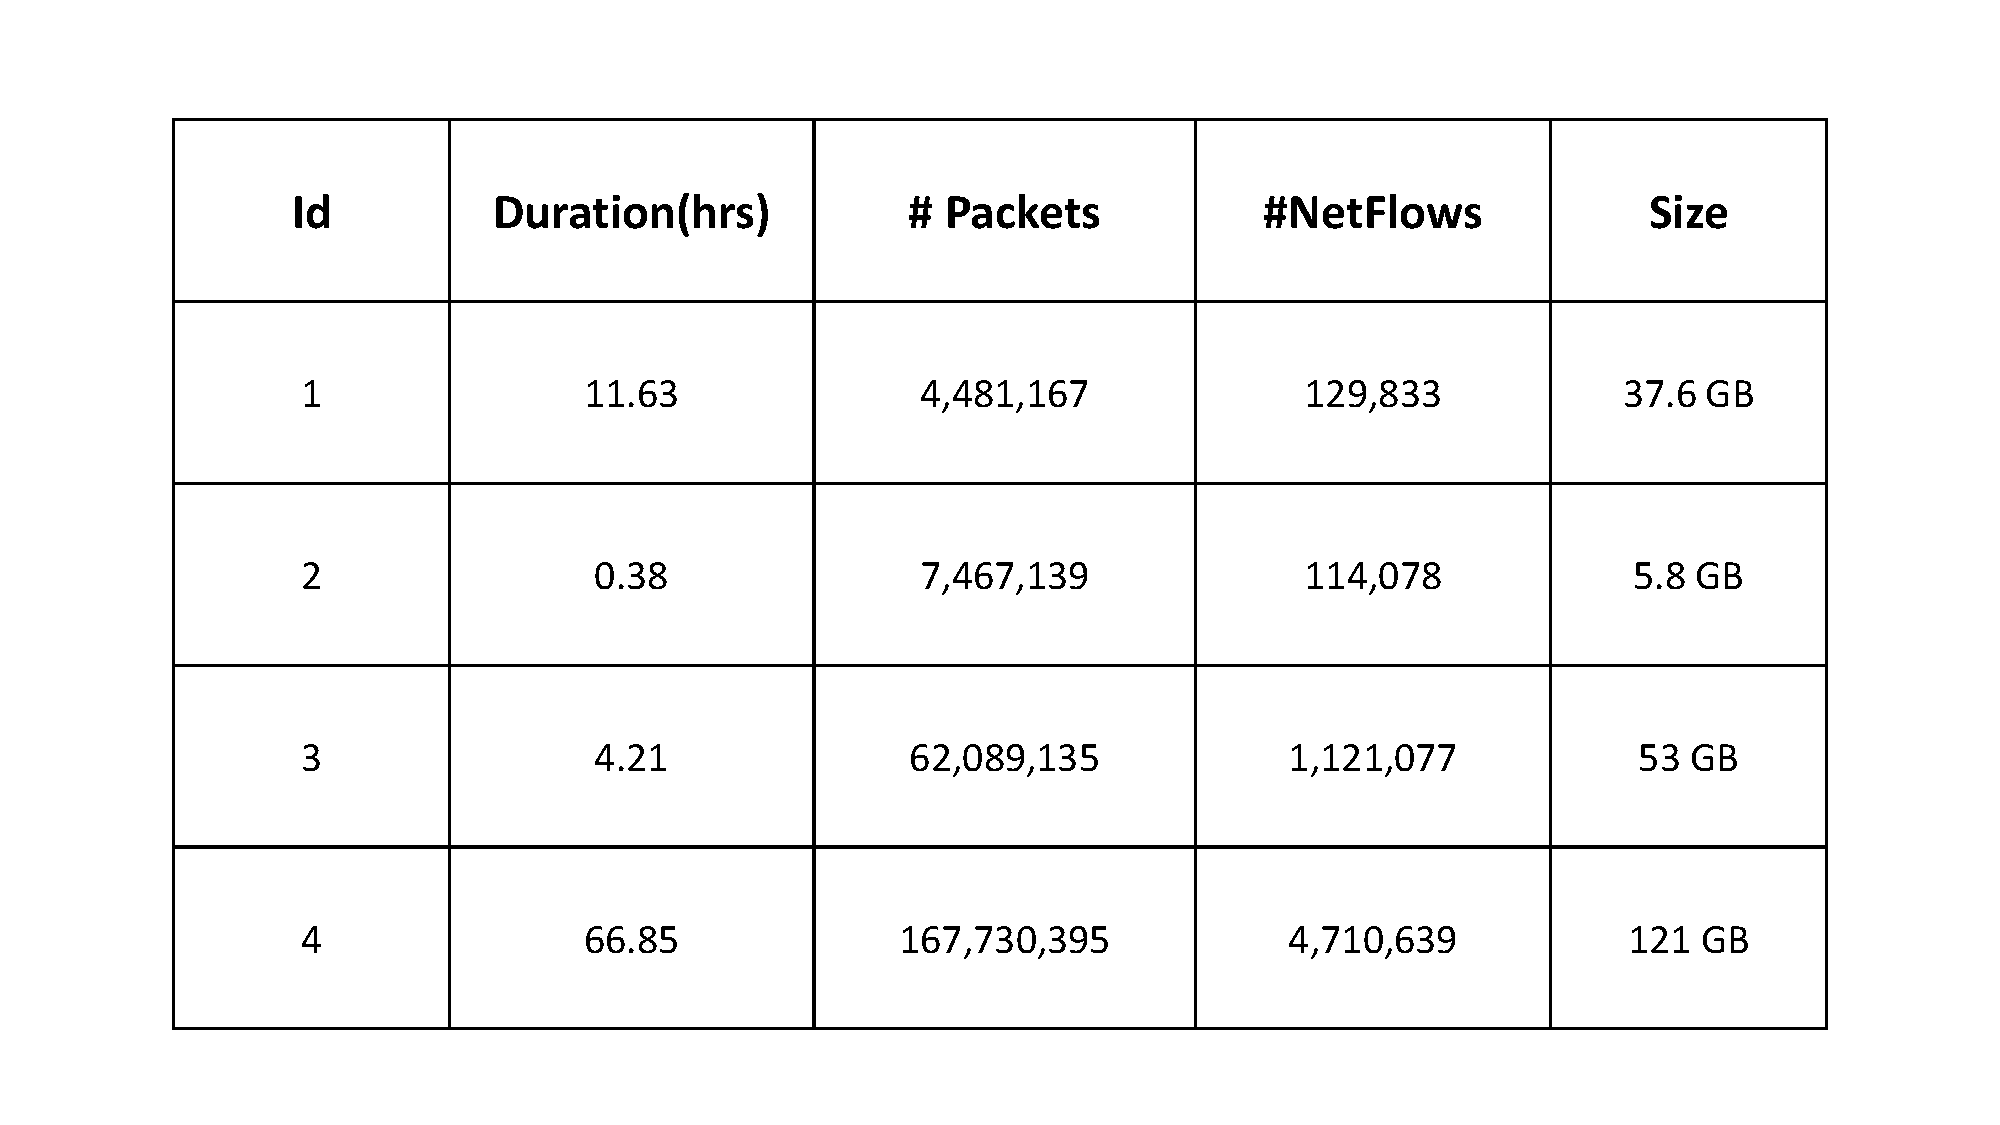
\includegraphics[scale = 0.5]{synth_desc.pdf}}	
	\tablabel{synthdesc}
\end{table}

The distinctive character of this data set is that each scenario is manually examined and labeled. After labeling the data set looks similar to the one which we capture at the emulab router excpet for the last column where the flow is labeled which can be seen in the \figref{ss_labeled}.

\begin{figure}[b]
	\centerline{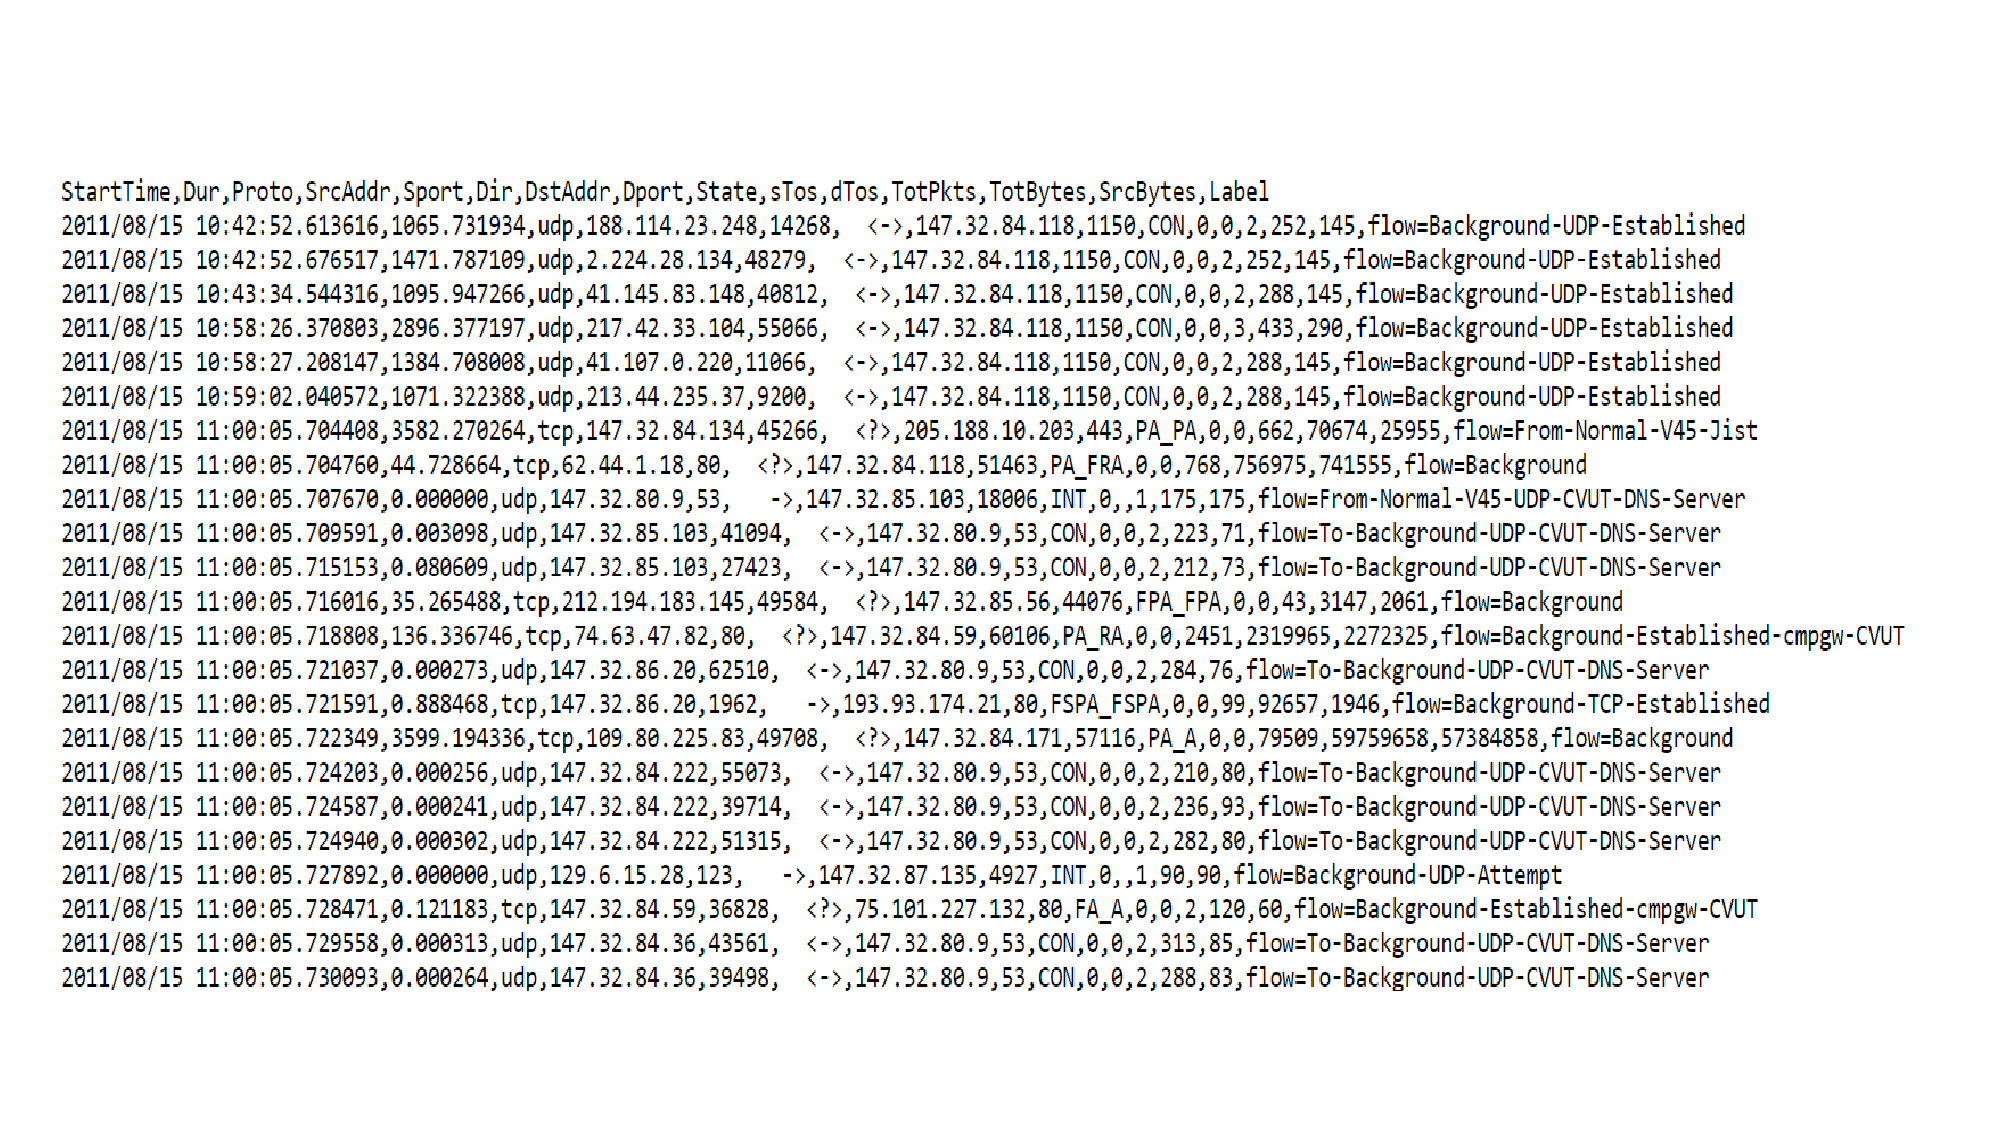
\includegraphics[trim=4cm 3cm 3cm 3cm, scale = 0.5]{ss_labeled.pdf}}
	\caption{Manually labeled synthetic data.}%
	\figlabel{ss_labeled}
\end{figure}

As mentioned earlier in this section these four different scenarios contain real network traffic and synthesized data. In the first scenario data is simulated to reflect UDP and ICMP DDOS attacks, In the second one traffic patterns exhibited by Scanning web proxies is simulated, The third and fourth scenarios have user generated traffic that mimics the behavior of chinese hosts and multiple synchronized networks respectively. Using these different captures(scenarios) we evaluated our systems basic functionality such as how effectively our system is able to extract the host behaviors, the detection rate of the different possible attacks and how will it respond with scale (when there are multiple users on multiple networks communicating simultaneously). The results are as follows:

\subsection{Scenario 1:}
The scenario 1 is of duration 4.21 hours with 53 GB of data. This dataset contains four different classes of traffic as per the manual inspection and labeling.

\begin{itemize}
	
	
	\item We were able to extract different host behaviors of interest to network admin, here we are mentioning two of them, namely scanners and DNS Query Responses. The cluster that contains scanners have a high incoming traffic trying to infiltrate the
	network by scanning for open ports. The amount of packets and bytes transferred by hosts in this cluster is unsubstantial. The behavior exhibited by the hosts of this
	cluster can be used by the network admin to monitor the security of the network.
	The cluster that contains DNS Query Responses has heavy traffic aiming at a single
	port. Studying about this cluster behavior over time will give an edge in planning
	bandwidth of the network. The remarkable feature of our system is that it has extracted
	the above behaviors without any prior knowledge of the hosts in the system or the input Netflow data.
	\item We have observed that over periods of short intervals of time(few weeks), the number
	of clusters have remained fairly constant which indicates that there has been no
	rapid change in the behaviors exhibited by the hosts. And our system performed
	seemingly well by choosing a constant number of clusters at the stage of pattern
	detection. Figure \figref{constant} represents how the number of clusters formed for a months
	data are close to constant.
	
	
	
	\item  By mapping cluster behaviors of a given day with a reference day we were also able
	to compare host behaviors. These comparisons can help network admin in capacity
	planning, threat analysis and other network monitoring activities. We built a tool to analyze these host behaviors. 
	We provide network admin with an option to compare
	behaviors on two days as shown in figure \figref{compare_days}
	
	
\end{itemize}



\begin{figure}[t]
	\centerline{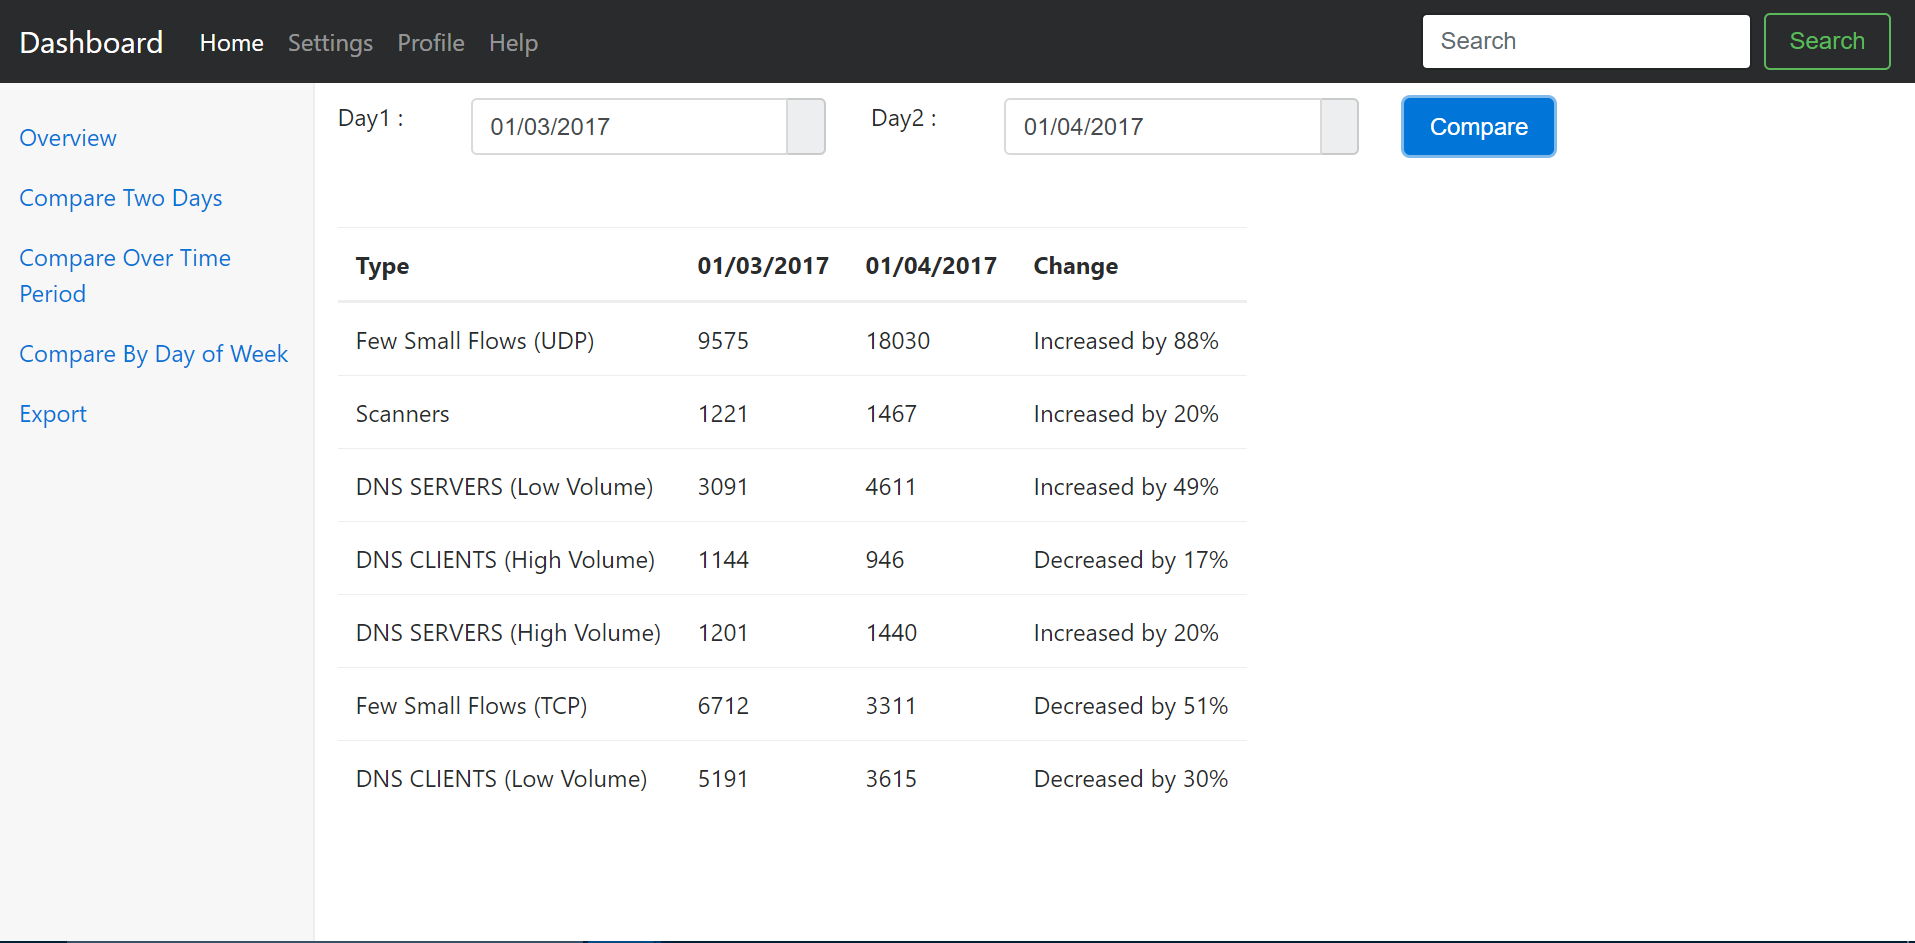
\includegraphics[scale = 0.45]{tool_compare_days.png}}
	\caption{Compare Host Behaviors on two days.}%
	\figlabel{compare_days}
\end{figure} 

The figure \figref{compare_weeks} gives an insight of how hosts behavior is changing over a month.
In the graph each line represents different host behaviors. The X-axis and Y-axis
represent the date on which this host behavior is observed and the number of hosts
which exhibited this behavior respectively.

\begin{figure}[t]
	\centerline{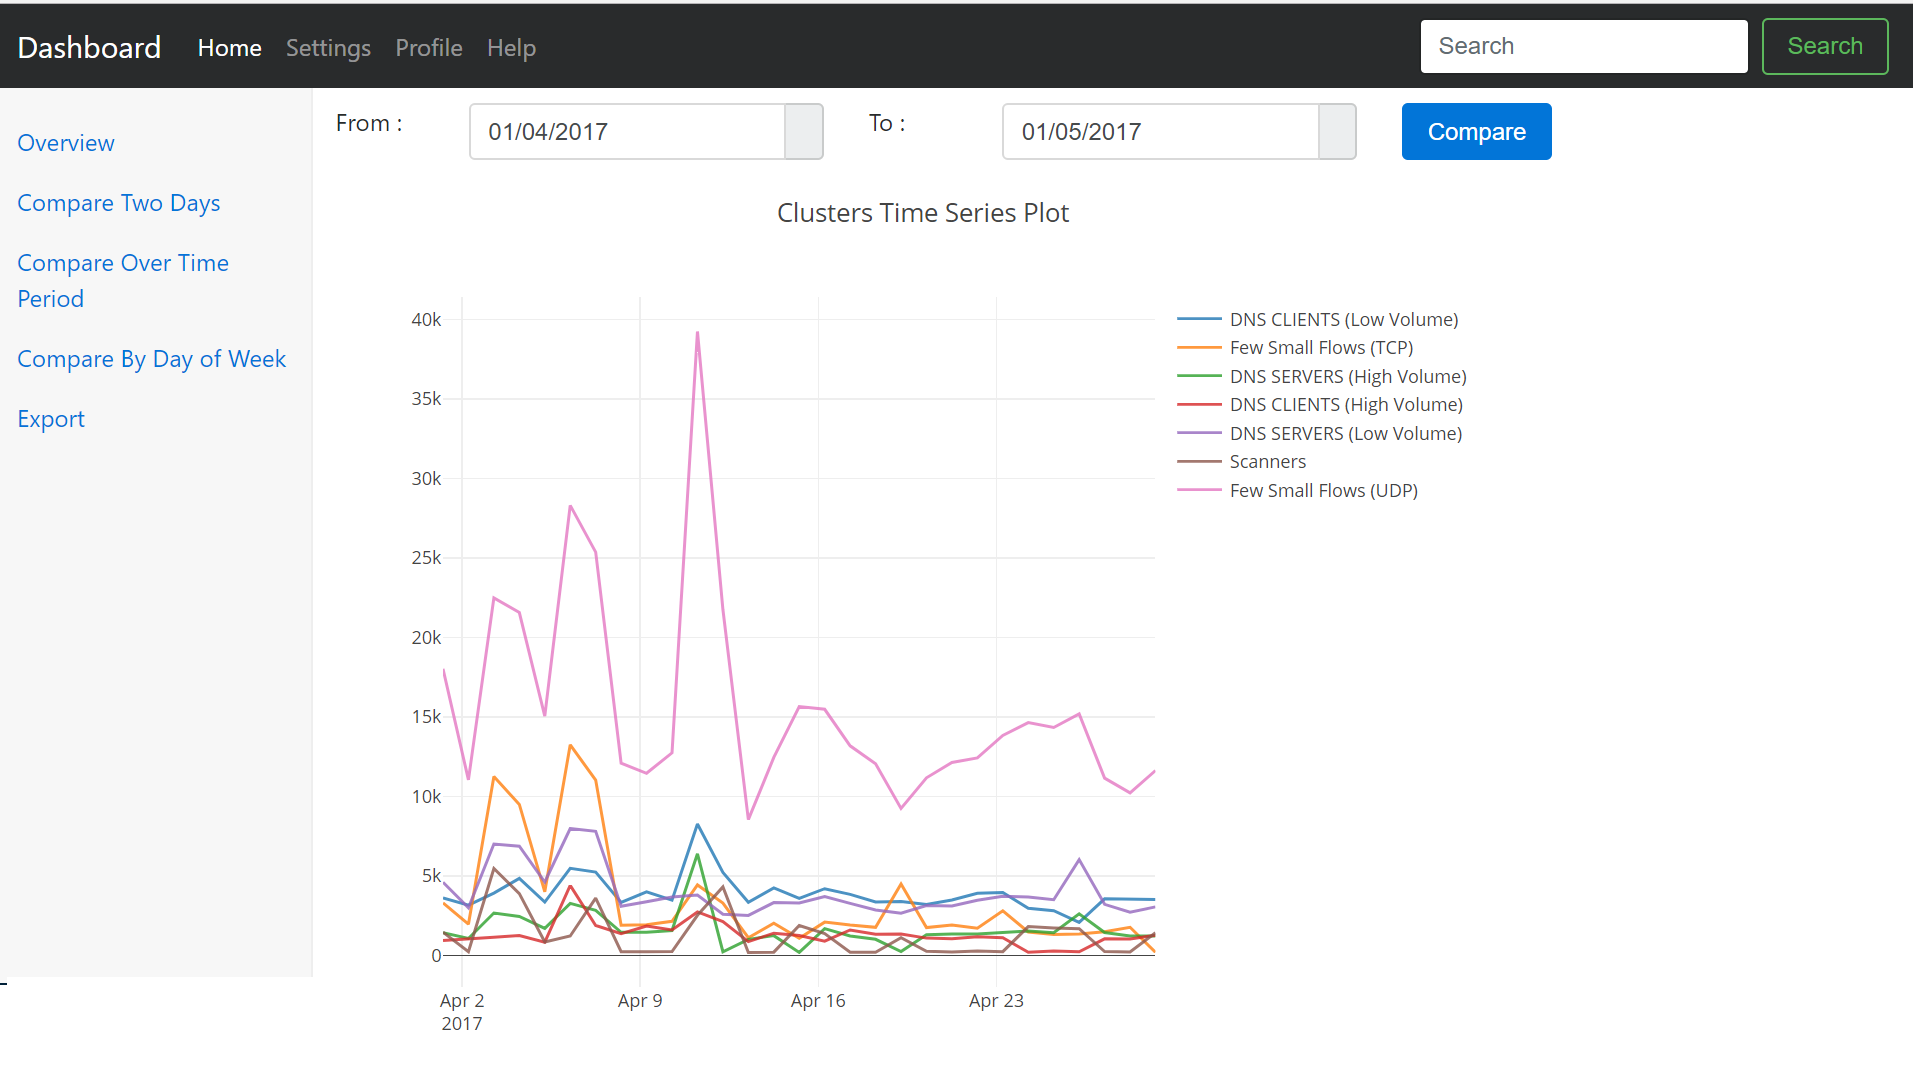
\includegraphics[scale = 0.45]{tool_compare_week.png}}
	\caption{Compare Host Behaviors over a time period.}%
	\figlabel{compare_weeks}
\end{figure} 



\section{Evaluation}

\tabref{evaluation} shows the planned evaluations of our sytsem which will be included in the final thesis defense.

\begin{table}[b]
	\caption{Planned Evaluations}%
	\centerline{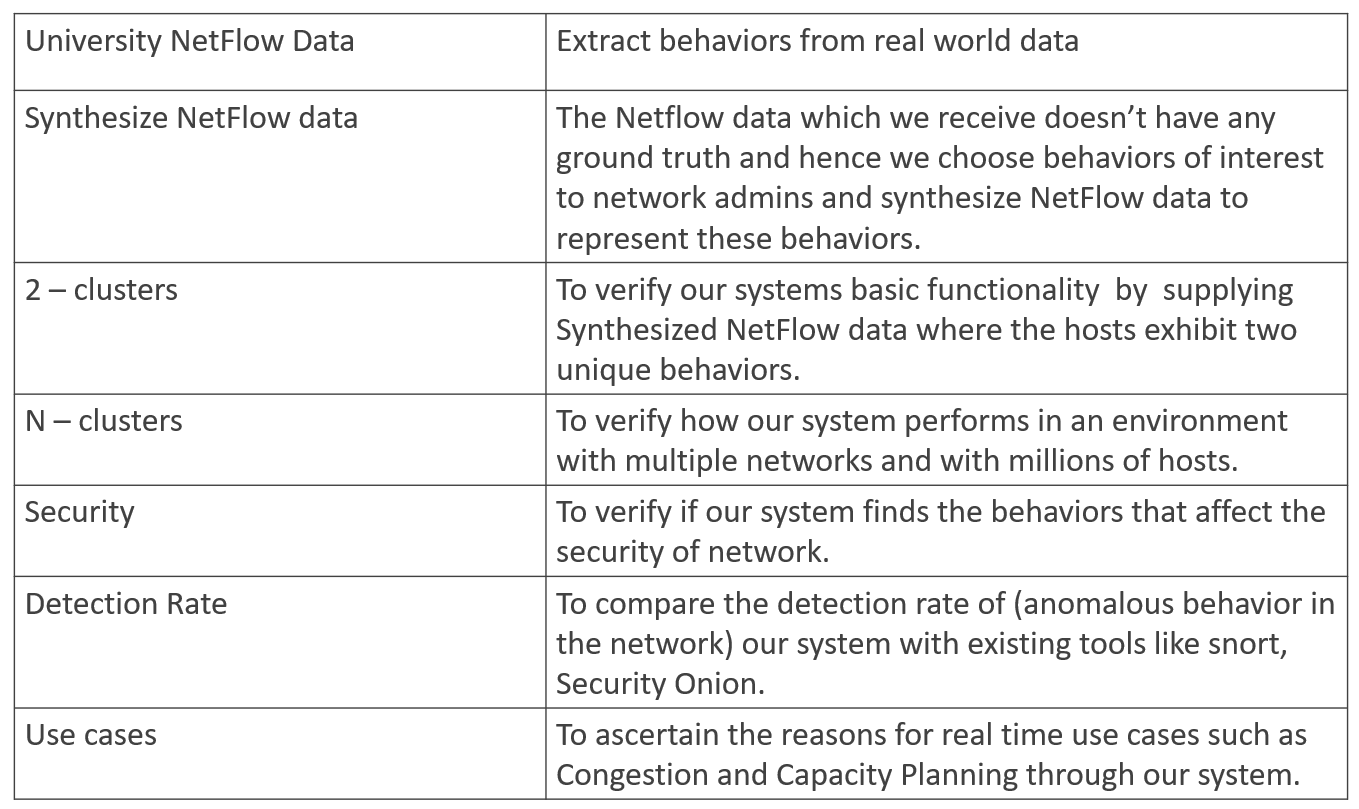
\includegraphics[scale = 0.6]{evaluation.png}}
	\tablabel{evaluation}
\end{table}


As Netflow data is unlabeled it gets tough to test few functionalities of the system
that we have built. Hence, in order to overcome this we want to insert some behaviors
into the NetFlow data(create simulated environment) and verify if our system is able to
detect them. Even with simulated environment one has to remember that we are not going
to provide any information pertaining to the behaviors of the hosts of the system or the
simulated data yet our system is expected to uncover them. In addition to this we will also
present set of results using real data.




The two main functionalities that we would like to test are :
\begin{itemize}
	
	\item Detecting the anomalous hosts in the network through host behaviors and find other
	such hosts that are of interest to security of network.
	
	\item Helping network administrator to efficiently predict the capacity needs of the network.
\end{itemize}

We would like to create a micro benchmark using the existing NetFlow analysis tools
for both the above scenarios. For the first scenario, we synthesize flow data that has
scanners trying to enter the system along with the web traffic(Http requests, DNS requests
and others..) and pass it through the existing tools. We expect these tools to give a detailed
sketch about the traffic based on applications and ports. But, when the same traffic is
passed through our system the expected output is at least two clusters one with normal
web traffic and the other with scanners. This is the important point that we would like to
mention about our system that is it extracts the information that we have never asked it to
look for.
Before talking about the second scenario, let us see how the state-of-art network analysis
tools perform bandwidth management. Solarwinds is an organization that provides
Network Management softwares. One of it’s licensed products is ”Netflow Traffic Analyzer
and Bandwidth monitoring software”. This tool works with Cisco NetFlow, Juniper
J-Flow, sFlow, Huawei NetStream, and IPFIX flow data and monitors bandwidth use by
application, protocol, and IP address group and identifies which applications, and protocols
are consuming the most bandwidth. So,our benchmark for second scenario would be
to synthesize flow data which needs more than an aggregation on application or protocol
to determine capacity needed for network and pass it through open source tools that use
similar bandwidth management techniques as Solarwinds. Similarly, on the other hand
we pass this data through our system and our expectation would be that we will be find
few clusters that will help admin understand which hosts are consuming the network
bandwidth and take suitable actions.